\documentclass[12pt,a4paper]{article}

%language and font
\usepackage[utf8]{inputenc}
\usepackage[english]{babel}
\usepackage[scaled]{beramono}
\usepackage[T1]{fontenc}

%% Useful packages
\usepackage{pdfpages}
\usepackage{amsmath}
\usepackage{mathrsfs}
\usepackage{amssymb}
\usepackage{graphicx}
\usepackage[colorinlistoftodos]{todonotes}
\usepackage[colorlinks=true, allcolors=blue]{hyperref}
\usepackage[left=2cm,right=2cm,top=2cm,bottom=2cm]{geometry}
\author{Y1471938}
\title{

\includegraphics[width=\textwidth]{images/yorkUniLogo.png}\\
\textbf{Systems programming for ARM}\\ extending DocetOS}

\begin{document}
\maketitle
\begin{abstract}
This document outlines the extensions and modifications made to the DocetOS operating system. The focus of the extensions is on scalability with the aim of allowing the extended docetOS to work with a large number of tasks efficiently. This results in a slight overhead in memory usage but allows for a priority scheduler that can efficiently switch between many tasks, and prevent starvation of individual tasks by ensuring that even the lowest priority task gets occasionally allocated CPU time (scheduling is stochastic, with the task priority determining the probability that the task will get selected). The scheduler incorporates an efficient task sleeping and waiting mechanism which aims to minimise the operations that have to be performed when a task transitions from one state to another. I have provided the user with tools to easily set up inter task communication through the OS channel manager, which is responsible for providing one or more tasks with access to the correct channel, and recycling the channel once the tasks no longer need it. In order to allow the user to easily allocate memory I have created a "memory cluster" that simultaneously aims to prevent memory being wasted and tasks having to wait for memory to become available. The memory provided by the cluster is guaranteed to be 8-byte aligned and can therefore also be used for task stacks. The OS itself uses the memory cluster to allocate the vast majority of its own internal resources such as hash tables, queues, heaps etc. All data structures used by the OS are standalone and available to the user for their own use. They come with convenience functions to quickly create and destroy them e.g "new\_hashtable(...)" allocates and initialises a hash table with the desired size.
\end{abstract}
\pagebreak
\tableofcontents
\pagebreak
\section{Coding Standard}

\section{The Stochastic Scheduler}
My plan was to allow DocetOS to support a large number of tasks, which made me come up with the following key requirements for the priority scheduler:
\begin{itemize}
  \item The scheduler should be pre-emptive, but allow tasks enough time to run to avoid wasting CPU time on frequent context switching.
  \item CPU time allocated per task should be dependant on the tasks priority, but the highest priority task should not be the only task getting CPU time (not just standard Fixed priority pre-emptive scheduling behaviour where only the highest priority task is selected)
  \item Task starvation should be avoided, even the lowest priority task should have a non-zero probability of getting selected during task switch.
  \item Task switching and status changes of tasks should not result in a large overhead of CPU time.
\end{itemize}

\pagebreak
\subsection{Implementation}
At the end of this section you will find an example illustration of the internal state of the scheduler at a particular point in time. The scheduler contains 2 heaps and 5 hashtables which are used to keep track of the various states a task can be in, and allow quick access to any task no matter its state.

\begin{itemize}
  \item The \textbf{Scheduler Heap} is used by the scheduler to determine what task to select for execution. This heap can contain tasks that are active and tasks that are waiting, sleeping or have tasks that have run to completion (see highlight 1). Tasks that are not active are only moved/removed from the scheduler heap if they are encountered in the heap during task selection. This is done to save cpu time on operations that might be unnecessary, a task that goes to sleep might wake up long before the scheduler comes across it in the heap, so moving it to the sleep heap would only waste cpu cycles on restructuring the sleep and scheduler heaps. When the scheduler comes across a sleeping/waiting task it checks if this state is still applicable and only then moves the task to a different heap/hashtable.
  \item The \textbf{Sleep Heap} stores tasks that are sleeping and have been removed from the scheduler heap. In this heap the tasks position in the heap is not determined by its priority but by its remaining sleep time (highlight 2). The scheduler removes the first node, updates its remaining sleep time by referring to the time it started sleeping and checks if it has woken up, if it has it is added back to the scheduler heap and the process is repeated. If the first node has not woken up yet then none of the other nodes will have woken up either. This approach means only one sleeping node has to be updated.
  \item The \textbf{tasksInSchedulerHeapHashTable} keeps track of all the tasks currently present in the scheduler heap. Used to check what tasks have to be added back to the scheduler heap after wake/notify and which ones were never removed.
  \item The \textbf{activeTasksHashTable} keeps track of all tasks that are currently executable.
  \item The \textbf{waitingTasksHashTable\_reasonAsKey/\_tcbAsKey} both keep track of tasks that are waiting. The \_reasonAsKey table is used during notify to change the state of a task waiting for "reason" without needing to check each waiting task. the \_tcbAsKey allows the OS and user to check if a given task is waiting.
  \item The  \textbf{sleepingTasksHashTable} keeps track of all tasks that are sleeping, no matter what heap they are in.
  \item The  \textbf{nodeContentIndexHashTable} internal (optional) hashtable of heap data structure, can be used to quickly determine at what index a node with a specific content is located in the heap. This is used during priority inheritance.
\end{itemize}

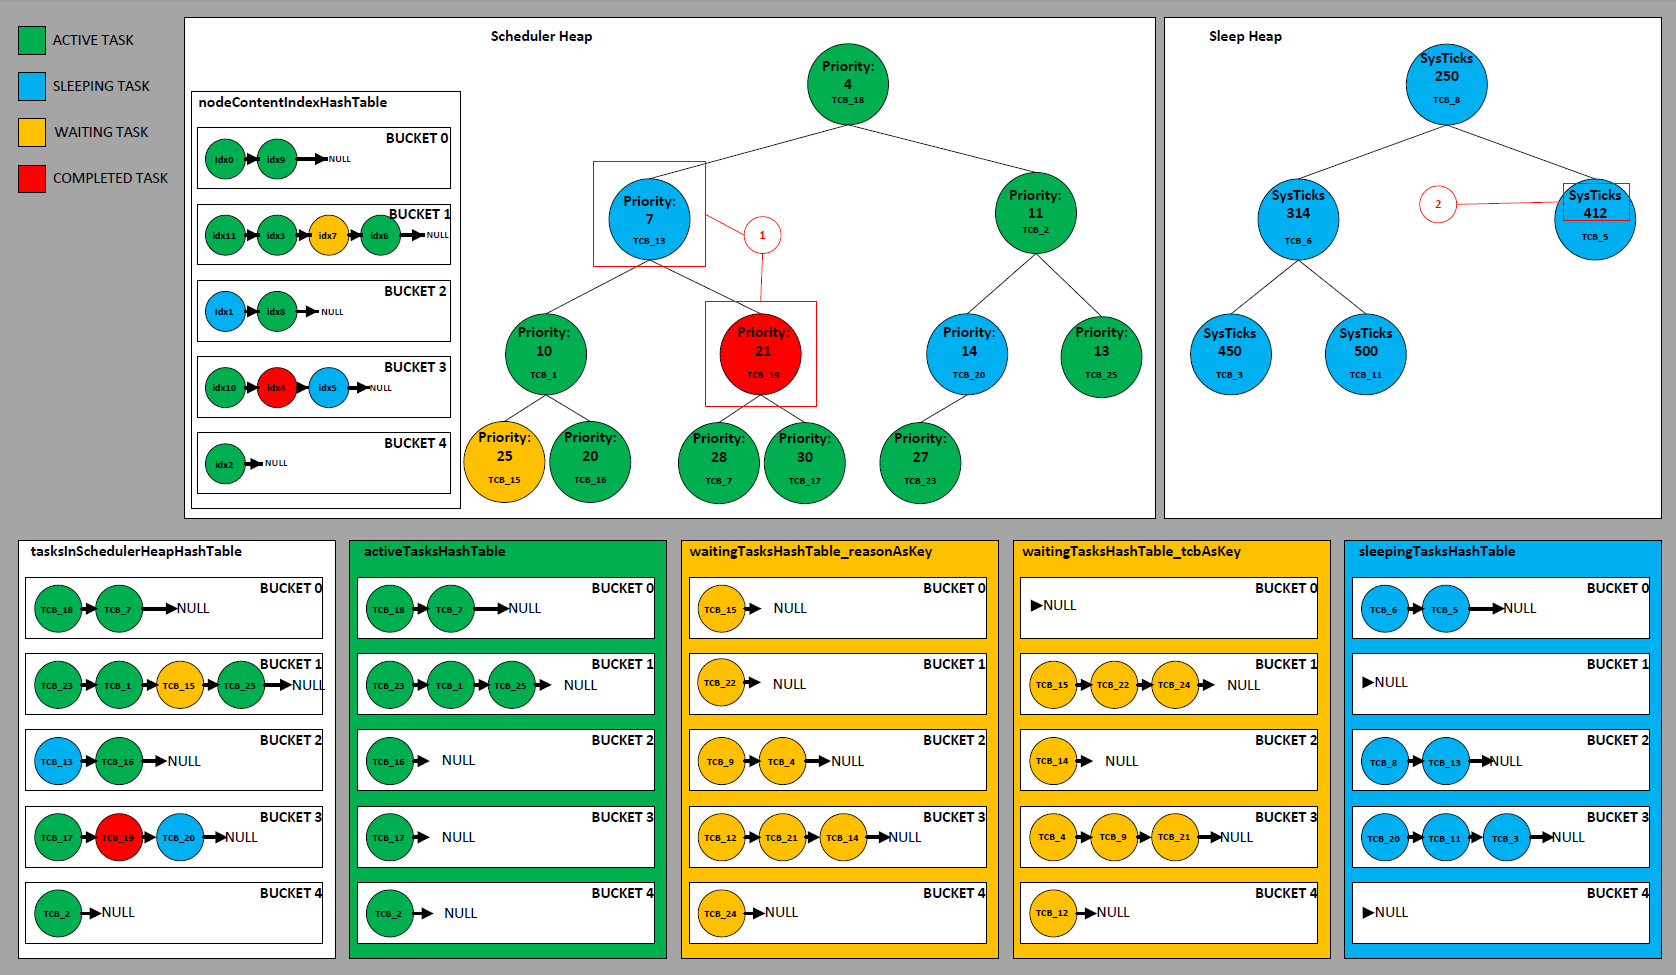
\includepdf[landscape=true]{images/schedulerOverview.png}


\subsection{Selecting a Task}
\subsection{Sleep}
\subsection{Wait}
\subsection{Notify}

\section{The Memory Cluster}
\subsection{Design Overview}
\subsection{Initialisation Process}
\subsection{Internal Resources}

\section{The Channel Manager}
\subsection{Design Overview}
\subsection{The Channel}
\subsection{Initialisation Process}

\section{Data Structures}
\subsection{Mutex}
\subsection{Semaphore}
\subsection{Queue}
\subsection{Hashtable}
\subsection{Heap}

\section{Demonstration Code Overview}


%%\todo{bla bla \ldots} test  test test. bla bla test test
\end{document}